\newpage
\section{积分变换}
\subsection{Fourier变换}
\noindent \textbf{Fourier级数:}
$$\begin{aligned}
    [-L/2,L/2]\quad& f(x)=a_{0}+\sum_{n=1}^{\infty}(a_{n}\cos\frac{2\pi n}{L}x+b_{n}\sin\frac{2\pi n}{L}x)\\
    \text{正交性}\quad& a_{0}=\frac{1}{L}\int_{-L/2}^{L/2}f(x)dx\\
    &a_{n}=\frac{2}{L}\int_{-L/2}^{L/2}f(x)\cos\frac{2\pi n}{L}x,\quad b_{n}=\frac{2}{L}\int_{-L/2}^{L/2}f(x)\sin\frac{2\pi n}{L}xdx
\end{aligned}$$

Fourier级数就是按照如下本征值问题的解所构成的完备集展开
$$\begin{cases}
    y^{\prime\prime}(x)+\lambda y(x)=0\\
    y(-L/2)=y(L/2),\quad y^{\prime}(-L/2)=y^{\prime}(L/2)
\end{cases}$$

\noindent \textbf{将$\sin,\cos$写成复数形式}
$$\cos\theta=\frac{e^{i\theta}+e^{-i\theta}}{2},\quad\sin\theta=\frac{e^{i\theta}-e^{-i\theta}}{2i}$$
$$\begin{aligned}
    f(x)=&a_{0}+\sum_{n=1}^{\infty}a_{n}\frac{e^{i\frac{2\pi n}{L}x}+e^{-i\frac{2\pi n}{L}x}}{2}+\sum_{n=1}^{\infty}b_{n}\frac{e^{i\frac{2\pi n}{L}x}-e^{-i\frac{2\pi n}{L}x}}{2i}\\
    =&a_{0}+\sum_{n=1}^{\infty}\frac{1}{2}(a_{n}-ib_{n})e^{i\frac{2\pi n}{L}x}+\sum_{n=1}^{\infty}\frac{1}{2}(a_{n}+ib_{n})e^{-i\frac{2\pi n}{L}x}\\
    =&\sum_{n=-\infty}^{\infty}c_{n}e^{i\frac{2\pi n}{L}x}
\end{aligned}$$

其中,系数$c_n$满足
$$c_n=\frac1L\int_{-L/2}^{L/2}f(x)e^{-\mathrm{i}\frac{2n\pi}Lx}\mathrm{d}x$$

或者将Fourier级数写成复数形式:
$$f(x)=\sum_{n=-\infty}^\infty c_ne^{\frac{2n\pi\mathrm{i}}Lx}$$

正交性:
$$\int_{-L/2}^{L/2}(e^{i\frac{2\pi m}{L}x})^{*}e^{i\frac{2\pi n}{L}x}dx=\begin{cases}{L,}&{m=n}\\{0,}&{m\neq n}\end{cases}$$

\noindent \textbf{令区间长度 $L\to\infty$, 将级数变成积分}
$$\begin{aligned}
    f(x)=&\sum_{k=\frac{2\pi}{L}n}\frac{1}{L}F(k)e^{ikx}\quad n=0,\pm1,\pm2,...\\\
    =&\frac{1}{2\pi}\sum_{k=\frac{2\pi}{L}n}\frac{2\pi}{L}F(k)e^{ikx}\\
    \xRightarrow{L\to\infty}&\frac{1}{2\pi}\int_{-\infty}^{+\infty}F(k)e^{ikx}dk
\end{aligned}$$

\begin{dfn}[Fourier变换]
    $$\boxed{F(k)=\mathscr{F}[f(x)]\equiv\int_{-\infty}^\infty f(x)\operatorname{e}^{-\operatorname{i}kx}\operatorname{d}x}$$
\end{dfn}

\begin{dfn}[Fourier逆变换]
    $$\boxed{f(x)=\mathscr{F}^{-1}[F(k)]\equiv\frac1{2\pi}\int_{-\infty}^\infty F(k)\operatorname{e}^{\operatorname{i}kx}\operatorname{d}k}$$
\end{dfn}

\noindent 为使变换\textbf{存在且可逆},要求:
\begin{enumerate}
    \item 任意有限区间上,$f(x)$分段光滑
    \item $f(x)$在$(-\infty,\infty)$上绝对可积,即$\int_{-\infty}^{\infty}|f(x)|dx<\infty\Rightarrow f(\pm\infty)\to 0$
\end{enumerate}

\subsubsection{Fourier变换的性质}
\begin{enumerate}
    \item 线性:$c_1f_1(x)+c_2f_2(x)\longleftrightarrow c_1F_1(k)+c_2F_2(k)$
    \item 微分公式:$f'(x)\longleftrightarrow ikF(k)\Rightarrow f^{(n)}(x)\longleftrightarrow (ik)^nF(k)$
    \item 卷积公式:$f*g(x)\longleftrightarrow F(k)G(k)$
\end{enumerate}
\begin{prf}[微分公式]
    $$\mathscr{F}[f(k)]=\int_{-\infty}^{+\infty}f(x)e^{-ikx}dx=e^{-ikx}f(x)\bigg|_{-\infty}^{+\infty}+ik\int_{-\infty}^{+\infty}f(x)e^{-ikx}dx=ik\int_{-\infty}^{+\infty}f(x)e^{-ikx}dx$$
\end{prf}
\begin{dfn}[卷积]
    $$a={a_0,a_1,...,a_n},b={b_0,b_1,...,b_n}$$
$$\begin{aligned}
    a\longleftrightarrow&f_a(t)=a_0+a_1t+...+a_nt_n\\
    b\longleftrightarrow&f_b(t)=b_0+b_1t+...+b_nt_n
\end{aligned}$$
$$\begin{aligned}
    f_a(t)f_b(t)=&a_0b_0+(a_0b_1+a_1b_0)t+...\\
    \equiv&c_0+c_1t+...+c_nt^n\\
    \equiv&f_{a*b}
\end{aligned}$$

    $$\boxed{f*g=\int_{-\infty}^{\infty}f(\xi)g(x-\xi)d\xi}$$
\end{dfn}
\begin{ex}[卷积的实际应用]
    两个独立连续随机变量$X,Y$,概率密度为$f_X(x),f_Y(y),Z=X+Y$的概率密度为
$$f(z)=\int_{-\infty}^{\infty}f_X(t)f_Y(z-t)dt$$
\end{ex}

\subsubsection{高维Fourier变换}
三维$\vec{r}=(x,y,z),\vec{k}=(k_x,k_y,k_z)$
$$$$
\subsubsection{Fourier变换的应用}
\begin{ex}[一维无限热传导]
    $$\begin{cases}
        \frac{\partial u}{\partial t}-k\frac{\partial^2 u}{\partial x^{2}}=0, \quad-\infty<x<\infty, \quad t>0\\
        u|_{t=0}=\phi(x)
    \end{cases}$$
    $$\int_{-\infty}^{+\infty}(\frac{\partial u}{\partial t}-k\frac{\partial^{2}u}{\partial x^{2}})e^{-ikx}dk=0$$
    $$\Rightarrow
    \begin{cases}
        \frac{\mathrm{d}U(k,t)}{\mathrm{d}t}+\kappa k^{2}U(k,t)=0\\
        U|_{t=0}=\mathscr{F}[\phi(x)]\equiv\Phi(k)
    \end{cases}$$
    $$U(k,t)=\Phi(k)e^{-\kappa k^{2}t}$$
    

    对两项分别做傅里叶逆变换:
    $$\begin{aligned}
        &\mathscr{F}^{-1}(\Phi(k))=\phi(x)\\
        &\mathscr{F}^{-1}(e^{-Kk^{2}t})=\frac{1}{2\pi}\int_{-\infty}^{+\infty}e^{-\kappa k^{2}t}e^{ikx}dk=\sqrt{\frac{\pi}{\kappa t}}e^{-\frac{x^{2}}{4\kappa t}}
    \end{aligned}$$

    $u$为两项逆变换的卷积
    $$\begin{aligned}
        u(x,t)&=\mathscr{F}^{-1}[\Phi(k)e^{-\kappa k^{2}t}]\\
        &=\int_{-\infty}^{+\infty}\phi(\xi)\frac{1}{2\sqrt{\pi \kappa t}}e^{-\frac{(x-\xi)^{2}}{4kt}}d\xi
    \end{aligned}$$

    \noindent\textbf{类比Fourier变换法和分离变量法}
    $$\begin{array}{cccc}
        \frac{2\pi n}{L}&T_{n}^{\prime}(t)+k(\frac{2\pi n}{L})^{2}T_{n}(t)=0    &&u=\sum_{n}X_{n}(x)T_{n}(t)\\
        k&\frac{dU(t,t)}{dt}+kR^{2}U(t,t)=0         &&u=\frac{1}{2\pi}\int\Phi(t)e^{-\kappa R^{2}t}dR
    \end{array}$$
\end{ex}

\begin{ex}[非齐次方程]
    $$\begin{cases}
        \frac{\partial u}{\partial t}-\kappa\frac{\partial^{2}u}{\partial x^{2}}=f(x,t)&-\infty<x<\infty,t>0\\
        u|_{t=0}=0
        \end{cases}$$

做Fourier变换$u(x,t)\longleftrightarrow U(k,t)\quad f(x,t)\longleftrightarrow F(k,t)$
$$\begin{cases}
    \frac{dU(k,t)}{dt}+\kappa k^{2}U(k,t)=F(k,t)\\
    U|_{t=0}\end{cases}$$

    根据齐次化原理:
$$U(k,t)=\int_{0}^{t}e^{-\kappa k^{2}(t-\tau)}F(k,\tau)d\tau$$
$$\begin{aligned}
    u(x,t)&=\mathscr{F}^{-1}\left[\int_{0}^{t}e^{-k^{2}(t-\tau)}F(k,\tau)d\tau\right]\\
    &=\int_{0}^{t}d\tau\mathscr{F}^{-1}\left[e^{-\kappa ^{2}(t-\tau)}F(k,\tau)\right]
\end{aligned}$$
分别对$e^{-\kappa ^{2}(t-\tau)},F(k,\tau)$求逆变换,再求卷积
$$\mathscr{F}(e^{-\kappa ^{2}(t-\tau)})=\frac{1}{2\sqrt{\pi \kappa(t-\tau)}}e^{-\frac{x^{2}}{4\kappa(t-\tau)}}$$
$$u(x,t)=\frac{1}{2\sqrt{\pi\kappa}}\int_{0}^{t}d\tau\int_{-\infty}^{+\infty}d\xi f(\xi,\tau)\frac{1}{\sqrt{t-\tau}}e^{-\frac{(x-\xi)^{2}}{4\kappa(t-\tau)}}$$
\end{ex}

\begin{ex}[三维齐次热传导问题]
    $$\begin{cases}
        \frac{\partial u}{\partial t}-k\nabla^2u=0&-\infty<x,y,z<\infty,t>0\\
        u|_{t=0}=\phi(\vec{r})&\vec{r}=(x,y,z)
    \end{cases}$$
    $$U(\vec{k},t)=\Phi(\vec{k})e^{-\kappa\vec{k}^{2}t}$$
分别对$e^{-\kappa\vec{k}^{2}t},\Phi(\vec{k})$求逆变换,再求卷积
$$\mathscr{F}(e^{-\kappa\vec{k}^{2}t})=\frac{1}{(4\pi \kappa t)^{3/2}}e^{-\frac{|\vec{x}-\vec{\xi}|^{2}}{4\kappa t}}$$
$$u(\vec{r},t)=\frac{1}{(4\pi \kappa t)^{3/2}}\iiint_{-\infty}^{\infty}\phi(\vec{\xi})e^{-\frac{|\vec{x}-\vec{\xi}|^{2}}{4\kappa t}}d\xi^{3}$$
\end{ex}


\newpage
\subsection{Laplace变换}
\begin{dfn}[Laplace变换]
    $$L[x(t)]=X(p)=\int_0^{\infty}{x(t)e^{-pt}dt }$$
\end{dfn}

\begin{dfn}[Laplace逆变换]
    $$x(t)=L^{-1}[X(p)]=\frac{1}{2πj}\int_{\sigma+j\infty}^{\sigma-j\infty}X(p)e^{pt}ds$$
\end{dfn}

只关心$t>0$:$f(t)$理解为$f(t)H(t)$,其中
$$H(t)=\begin{cases}
1 &t\ge0\\
0 &t<0
\end{cases}$$

收敛性优于Fourier变换

\subsubsection{Laplace变换的性质}
\begin{figure}[htpb]
    \centering 
    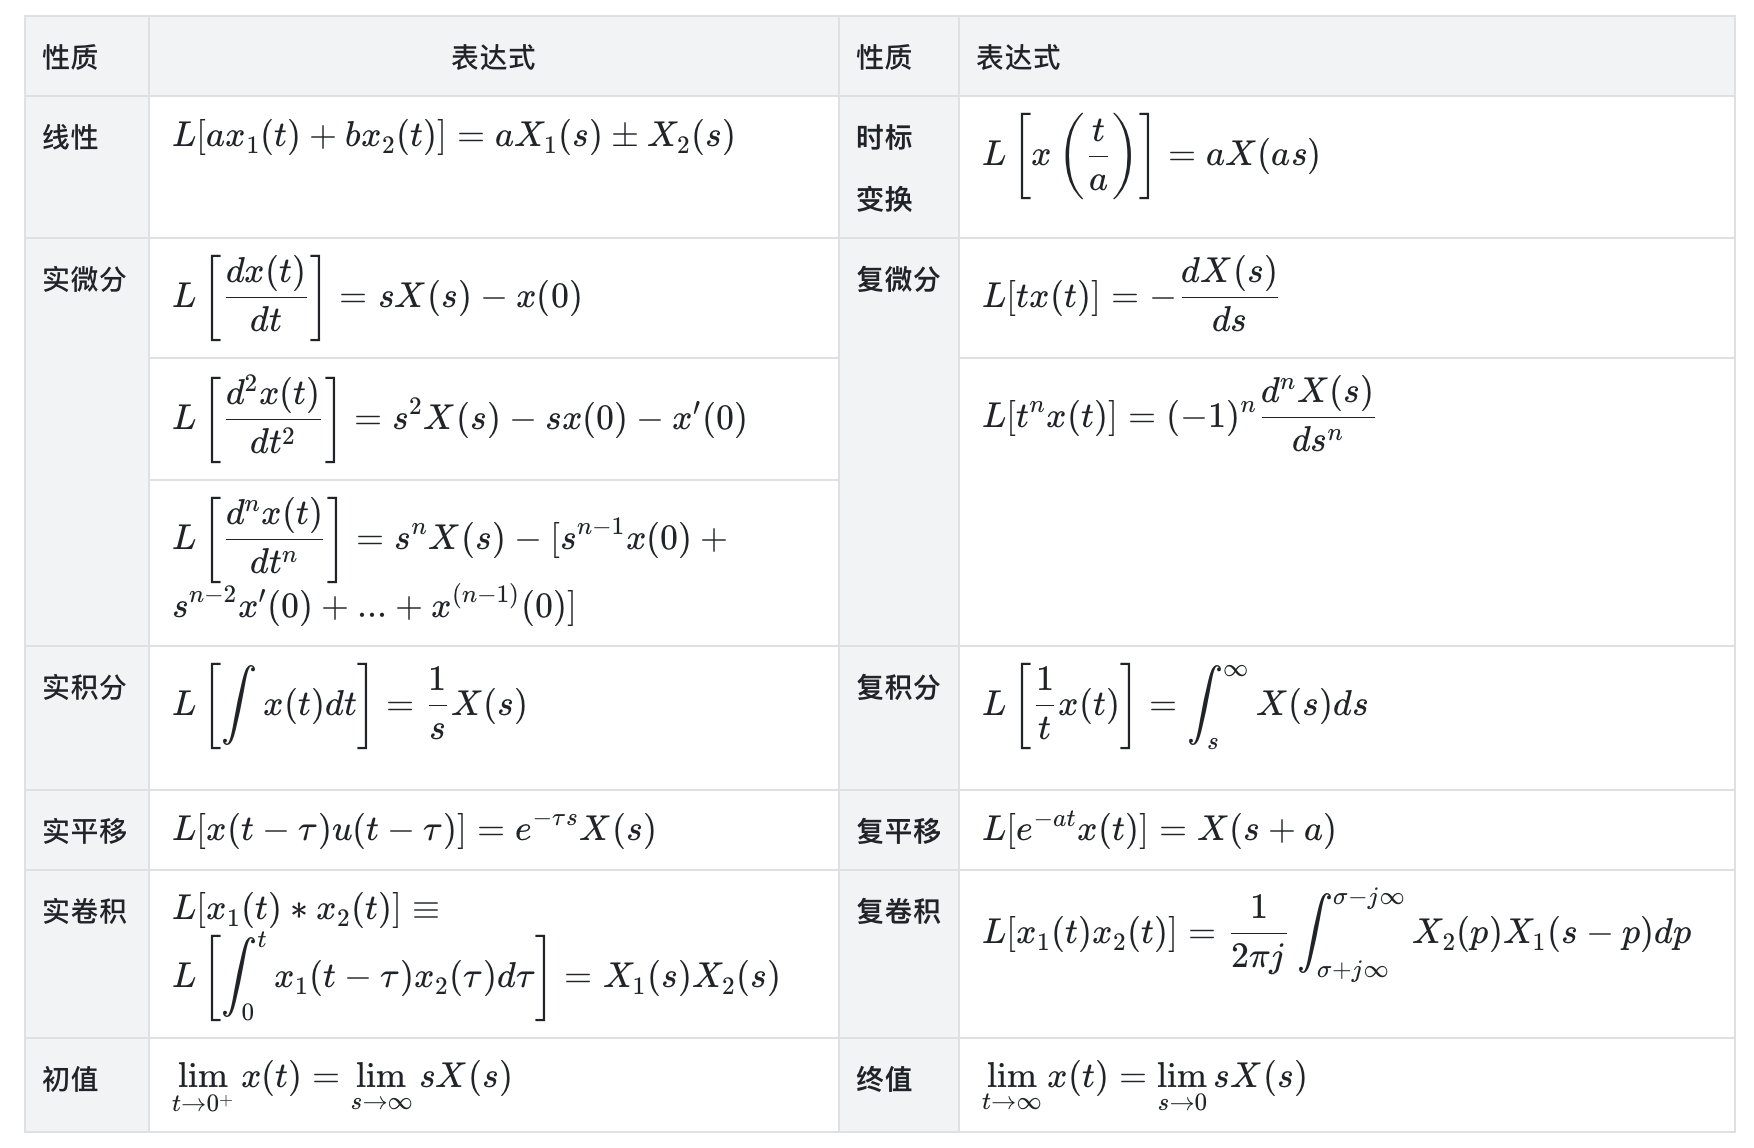
\includegraphics[width=16.5cm]{figures/LaplaceTransformProperties.png} 
    \caption{Laplace变换的性质}
    \label{LaplaceTransformProperties}
\end{figure}

\newpage
\subsubsection{常用函数的Laplace变换}
\begin{multicols}{2}
    $$\begin{aligned}
        &f(t)&&\mathcal{L}[f(t)]=F(s)\\
        &1&&\frac1s\\
        &e^{-at}f(t)&&F(s+a)\\
        &\mathcal{U}(t-a)&&\frac{e^{-as}}s\\
        &f(t-a)\mathcal{U}(t-a)&&e^{-as}F(s)\\
        &\delta(t)&&1\\
        &\delta(t-t_0)&&e^{-st_0}\\
        &t^nf(t)&&(-1)^n\frac{d^nF(s)}{ds^n}\\
        &f'(t)&&sF(s)-f(0)\\
        &f^n(t)&&s^nF(s)-s^{(n-1)}f(0)-\\
        &&&...-f^{(n-1)}(0)\\
        &\int_0^tf(x)g(t-x)dx\qquad&&F(s)G(s)\\
        &t^n\left(n=0,1,2,\ldots\right)&&\frac{n!}{s^{n+1}}\\
        &t^x\left(x\geq-1\in\mathbb{R}\right)&&\frac{\Gamma(x+1)}{s^{x+1}}\\
        &\sin kt&&\frac k{s^2+k^2}\\
        &\cos kt &&\frac s{s^2+k^2}\\
        &e^{at}&&\frac1{s-a}\\
        &\sinh kt&&\frac k{s^2-k^2}\\
        &\cosh kt&&\frac s{s^2-k^2}\\
        &\frac{e^{at}-e^{bt}}{a-b}&&\frac1{(s-a)(s-b)}
        \end{aligned}$$

        $$\begin{aligned}
            &f(t)&& \mathcal{L}[f(t)]=F(s)  \\
            &\frac{ae^{at}-be^{bt}}{a-b}&& \frac s{(s-a)(s-b)}  \\
            &te^{at}&& \begin{aligned}\frac{1}{(s-a)^2}\end{aligned}  \\
            &t^ne^{at}&& \frac{n!}{(s-a)^{n+1}}  \\
            &e^{at}\sin kt&& \frac k{(s-a)^2+k^2}  \\
            &e^{at}\cos kt&& \frac{s-a}{(s-a)^2+k^2}\\
            &e^{at}\sinh kt&& \frac k{(s-a)^2-k^2}  \\
            &e^{at}\cosh kt&& \frac{s-a}{(s-a)^2-k^2}  \\
            &t\sin kt&& \frac{2ks}{(s^2+k^2)^2}  \\
            &t\cos kt&& \frac{s^2-k^2}{(s^2+k^2)^2}  \\
            &t\sinh kt&& \frac{2ks}{(s^2-k^2)^2}  \\
            &t\cosh kt&& \frac{s^2-k^2}{(s^2-k^2)^2}  \\
            &\frac{\sin at}t&& \arctan\frac as  \\
            &\frac1{\sqrt{\pi t}}e^{-a^2/4t}&& \frac{e^{-a\sqrt s}}{\sqrt s}  \\
            &\frac a{2\sqrt{\pi t^3}}e^{-a^2/4t}&& e^{-a\sqrt{s}}  \\
            &\mathrm{erfc}\left(\frac a{2\sqrt{t}}\right)&& \frac{e^{-a\sqrt{s}}}s 
        \end{aligned}$$
    \end{multicols}



\subsubsection{Laplace变换的应用}
\begin{ex}[ODE:受迫振动]
    $$\begin{cases}y^{\prime\prime}(t)+w^{2}y(t)=f(t)\\y(0)=y'(0)=0\end{cases}$$

    $$p^2Y(p)-Py(0)-y^{\prime}(0)+w^2Y(p)=F(p)$$
    $$p^{2}Y(p)+w^{2}Y(p)=F(p)\Rightarrow Y(p)=\frac{1}{p^{2}+w^{2}}F(p)$$
对$\frac{1}{p^{2}+w^{2}},F(p)$两项分别做Laplace变换,然后做卷积。
$$L\left(\frac{1}{p^{2}+w^{2}}\right)=\frac{1}{\omega}\sin \omega t$$
$$y(t)=\int_{0}^{t}\frac{1}{w}\sin(t-\tau)f(\tau)d\tau $$
\end{ex}

\begin{ex}[半无界端点外力下的波动方程]
    $$\begin{cases}
        \frac{\partial^{2}u}{\partial t^{2}}=a^{2}\frac{\partial^{2}u}{\partial x^{2}}\quad x>0,\quad t>0\\
        \frac{\partial u}{\partial x}|_{x=0}=f(t)
        \\u|_{t=0}=\frac{\partial y}{\partial t}|_{t=0}=0
        \end{cases}$$
        $$\frac{\partial u}{\partial t^2}\longleftrightarrow p^2U-pu|_{t=0}-\frac{\partial u}{\partial t}\bigg|_{t=0}=p^2U$$
        $$\begin{cases}p^{2}U(x,p)=a^{2}\frac{d^{2}}{dx^{2}}U(x,p)\\\frac{dU}{dx}|_{x=0}=F(p),\quad U|_{x=+\infty}=0\end{cases}$$
        $$\begin{aligned}U(x,p)&=ce^{\frac{p}{a}x}+De^{-\frac{p}{a}x}\\&=-\frac{a}{p}e^{-\frac{p}{a}x}F(p)\end{aligned}$$

\noindent 法1:组合$-\frac{a}{p}e^{-\frac{x}{a}p}$;查表得$L^{-1}[\frac{1}{p}e^{-\lambda p}]=H(t-\lambda)$,令$\lambda=\frac xa$
        $$L^{-1}[-\frac{a}{p}e^{-\frac{x}{a}p}]=-aH(t-\frac{x}{a})$$
        $$\begin{aligned}
            u(x,t)
            &=L^{-1}[-\frac{a}{p}e^{-\frac{x}{a}p}F(p)]\\
            &=-a\int_{0}^{t}H(t-\tau-\frac{x}{a})f(\tau)d\tau\\
            &=\begin{cases}0,t<\frac{x}{a}\\-a\int_{0}^{t-\frac{x}{a}}f(\tau)d\tau,t\geq\frac{x}{a}\end{cases}\\
            &=-aH(t-\frac{x}{a})\int_0^{t-\frac{x}{a}}f(\tau)d\tau 
            \end{aligned}$$

\noindent 法2: 组合$-\frac{a}{p}F(p)$
$$\begin{aligned}L^{-1}[-\frac{a}{p}F(p)]&=-a\int_{0}^{t}f(\tau)d\tau\\L^{-1}[e^{-\lambda p}G(p)]&=g(t-\lambda)H(t-\lambda)\end{aligned}$$

取$\lambda=\frac{x}{a},\quad G(p)=-\frac{a}{p}F(p)$
$$\begin{aligned}L^{-1}[-\frac{a}{p}e^{-\frac{x}{a}p}F(p)]&=H(t-\frac{x}{a})g(t-\frac{x}{a})\\&=H(t-\frac{x}{a})(-a\int_{0}^{t-\frac{x}{a}}f(\tau)d\tau)\end{aligned}$$
\end{ex}